\documentclass[a4paper]{article}

\usepackage[a4paper, top=8mm, bottom=8mm, left=8mm, right=8mm]{geometry}

\usepackage{polyglossia}
\setdefaultlanguage[babelshorthands=true]{russian}
\setotherlanguage{english}

\usepackage{fontspec}
\setmainfont{FreeSerif}
\newfontfamily{\russianfonttt}[Scale=0.7]{DejaVuSansMono}

\usepackage[tiny, compact]{titlesec}

\usepackage{titling}
\setlength{\droptitle}{-1cm}
\pretitle{\begin{center}\begin{bfseries}\Large}
\posttitle{\par\end{bfseries}\end{center}}
\preauthor{\begin{center}\normalsize}
\postauthor{\par\end{center}\vspace{-1.8cm}}

\usepackage{hyperref}
\usepackage{bookmark}
\usepackage{csquotes}
\usepackage{graphicx}


\title{Экспериментальное ислледование методов оптимизации умножения плотных матриц на графических процессорах с использованием OpenCL}

\author{Грезин Данил Максимович}

\date{}

\begin{document}
\maketitle
\begin{flushright}
\begin{tabular}{r}
    Группа: \emph{\enquote{25.Б41-мм}} \\
    Кафедра: \emph{системного программирования} \\
    Научный руководитель: \emph{Григорьев Семен Вячеславович} \\
    Номер семестра практики: \emph{2} \\
\end{tabular}
\end{flushright}

\section{Постановка задачи}

Умножение плотных матриц с элементами одинарной точности (стандартный 32-битный формат представления чисел с плавающей точкой) является одной из наиболее важных вычислительных операций в высокопроизводительных вычислениях, поэтому производительность многих приложений напрямую зависит от эффективности ее реализации на графических процессорах.

Работа выполнялась в рамках учебного исследования методов оптимизации вычислений на графическом процессоре NVIDIA GeForce RTX 4060 с использованием технологии OpenCL на основе существующего набора реализаций умножения матриц. Реализации отличаются применяемыми методами повышения производительности, направленными на сокращение числа обращений к памяти, более эффективное использование локальной памяти и регистров, а также увеличение объема вычислений, выполняемых каждым потоком. Для ряда реализаций предусмотрены настраиваемые параметры, включая размеры вычислительных блоков, объем работы, выполняемой одним потоком, и ширину используемых векторов, значения которых могут существенно влиять на достигаемую производительность.

\textbf{Целью работы является} экспериментальное исследование влияния различных методов оптимизации умножения матриц на производительность вычислений при их выполнении на графическом процессоре, а также автоматизация подборка параметров оптимизации и определение наиболее эффективной конфигурации для используемого графического процессора.

Результаты работы позволяют оценить эффективность отдельных оптимизаций и их вклад в итоговую производительность вычислений. Полученные данные могут использоваться для выбора оптимальных параметров реализации умножения матриц на конкретном графическом процессоре.

Для достижения поставленной цели были решены следующие задачи:
\begin{itemize}
\item провести экспериментальное исследование производительности различных реализаций умножения матриц, представленных в проекте myGEMM\footnote{Cedric Nugteren. Репозиторий проекта myGEMM. URL: \url{https://github.com/CNugteren/myGEMM} (дата обращения: 10.03.2026).};
\item проанализировать влияние отдельных методов оптимизации, используемых в реализациях умножения матриц, на производительность выполнения вычислений на графическом процессоре;
\item автоматизировать подбор параметров оптимизации;
\item определить оптимальные значения параметров для используемого графического процессора и сравнить их со значениями, предлагаемыми в проекте myGEMM по умолчанию.
\end{itemize}

\section{Описание предлагаемого решения}

В качестве основы для выполнения работы был использован проект myGEMM, реализующий набор методов оптимизации умножения матриц с использованием OpenCL.

В проекте myGEMM представлено 11 вариантов вычислительных ядер, каждое из которых реализует новый метод оптимизации умножения матриц. Наличие нескольких реализаций позволяет проследить влияние методов оптимизации на производительность вычислений на графическом процессоре и делает проект myGEMM удобной платформой для экспериментального исследования подходов к повышению эффективности вычислений.

В рамках работы были разработаны программы на языке Python, обеспечивающие автоматический запуск вычислительных ядер, сбор результатов измерений, их статистическую обработку и подбор оптимальных параметров. Все программы расположены в корневом каталоге проекта, разрабатываемого в рамках данной работы:

\begin{itemize}
\item \texttt{run\_experiments\_default.py}~--- запуск измерений с параметрами по умолчанию для каждого ядра;
\item \texttt{run\_experiments\_tuned.py}~--- перебор всех допустимых комбинаций параметров для каждого ядра с проверкой ограничений (объем памяти, делимость значений);
\item \texttt{calculate\_results\_default.py}~--- статистическая обработка результатов по умолчанию: расчет среднего, стандартного отклонения, 95\% доверительного интервала, проверка нормальности;
\item \texttt{calculate\_results\_tuned.py}~--- статистическая обработка результатов с перебором параметров и выбор лучшей конфигурации по наибольшему среднему значению производительности.
\end{itemize}

Для проверки корректности разработанных программ были написаны модульные тесты с использованием \texttt{pytest}, размещенные в директории \texttt{tests/unit/}. Тесты охватывают корректность функций проверки подбираемых параметров, статистической обработки результатов и обработки выбросов.

\section{Экспериментальное исследование производительности}

С использованием разработанных программ были проведены измерения производтиельности ядер myGEMM в стандартной и оптимизированной конфигурациях.

Эксперименты проводились на следующей конфигурации вычислительной системы:
\begin{itemize}
\item процессор AMD Ryzen 7 7435HS (8 ядер, 16 потоков);
\item оперативная память 16 ГБ;
\item графический процессор NVIDIA GeForce RTX 4060 Laptop GPU (8 ГБ);
\item операционная система Manjaro Linux;
\item драйвер NVIDIA 590.48.01;
\item CUDA Toolkit 13.1;
\item NVCC 13.1.115;
\item OpenCL 3.0;
\item компилятор GCC 15.2.1;
\item флаги компиляции \texttt{-O3 -arch=sm\_89 -Xcompiler -Wall}.
\end{itemize}

Для каждой конфигурации выполнялось 40 измерений производительности после серии предварительных запусков. Между компиляциями и сменами размеров матриц делалась пауза для стабилизации температурного режима графического процессора. В качестве исследуемой задачи использовалось умножение квадратных матриц размера \(8192 \times 8192\) (степень двойки) и \(8320 \times 8320\) (не степень двойки, для проверки ядер с поддержкой матриц, размеры которых не кратны размеру вычислительного блока). По результатам измерений вычислялись среднее значение производительности (GFLOPS), стандартное отклонение и 95\%-й доверительный интервал, а также выполнялась проверка нормальности распределения результатов с использованием тестов Д'Агостино и Шапиро-Уилка.

Время выполнения каждого измерения определялось с использованием функции \texttt{gettimeofday}, обеспечивающей получение времени в секундах. Каждый элемент результирующей матрицы при умножении плотных квадратных матриц размера \(N \times N\) вычисляется как скалярное произведение строки и столбца длины \(N\), что требует выполнения \(N\) операций умножения и \(N\) операций сложения. Таким образом, для вычисления одного элемента выполняется \(2N\) арифметических операций, а для всей результирующей матрицы, содержащей \(N^2\) элементов,~--- \(2N^3\) операций. Производительность измеряется в FLOPs (Floating-point Operations Per Second) как число арифметических операций с числами с плавающей точкой, выполняемых за единицу времени. Итоговая производительность вычислялась по формуле:
\[
GFLOPS = \frac{2N^3}{t \cdot 10^9},
\]
где \(t\)~--- время выполнения одного измерения в секундах.

Результаты измерений для базовой конфигурации, а также после автоматического подбора параметров представлены на странице репозитория в файле \texttt{README.md}.

Сравнение производительности ядер до и после подбора параметров для матриц приведено на рисунке~\ref{fig:kernel-comparison}. Бордовым и малиновым цветами показаны результаты выполнения через CUDA и OpenCL соответсвтенно, а белыми отрезками обозначено стандартное отклонение результатов измерений. Обозначение <<no changes>> означает, что параметры ядра по умолчанию уже являлись оптимальными.

\begin{figure}[htbp]
    \centering
    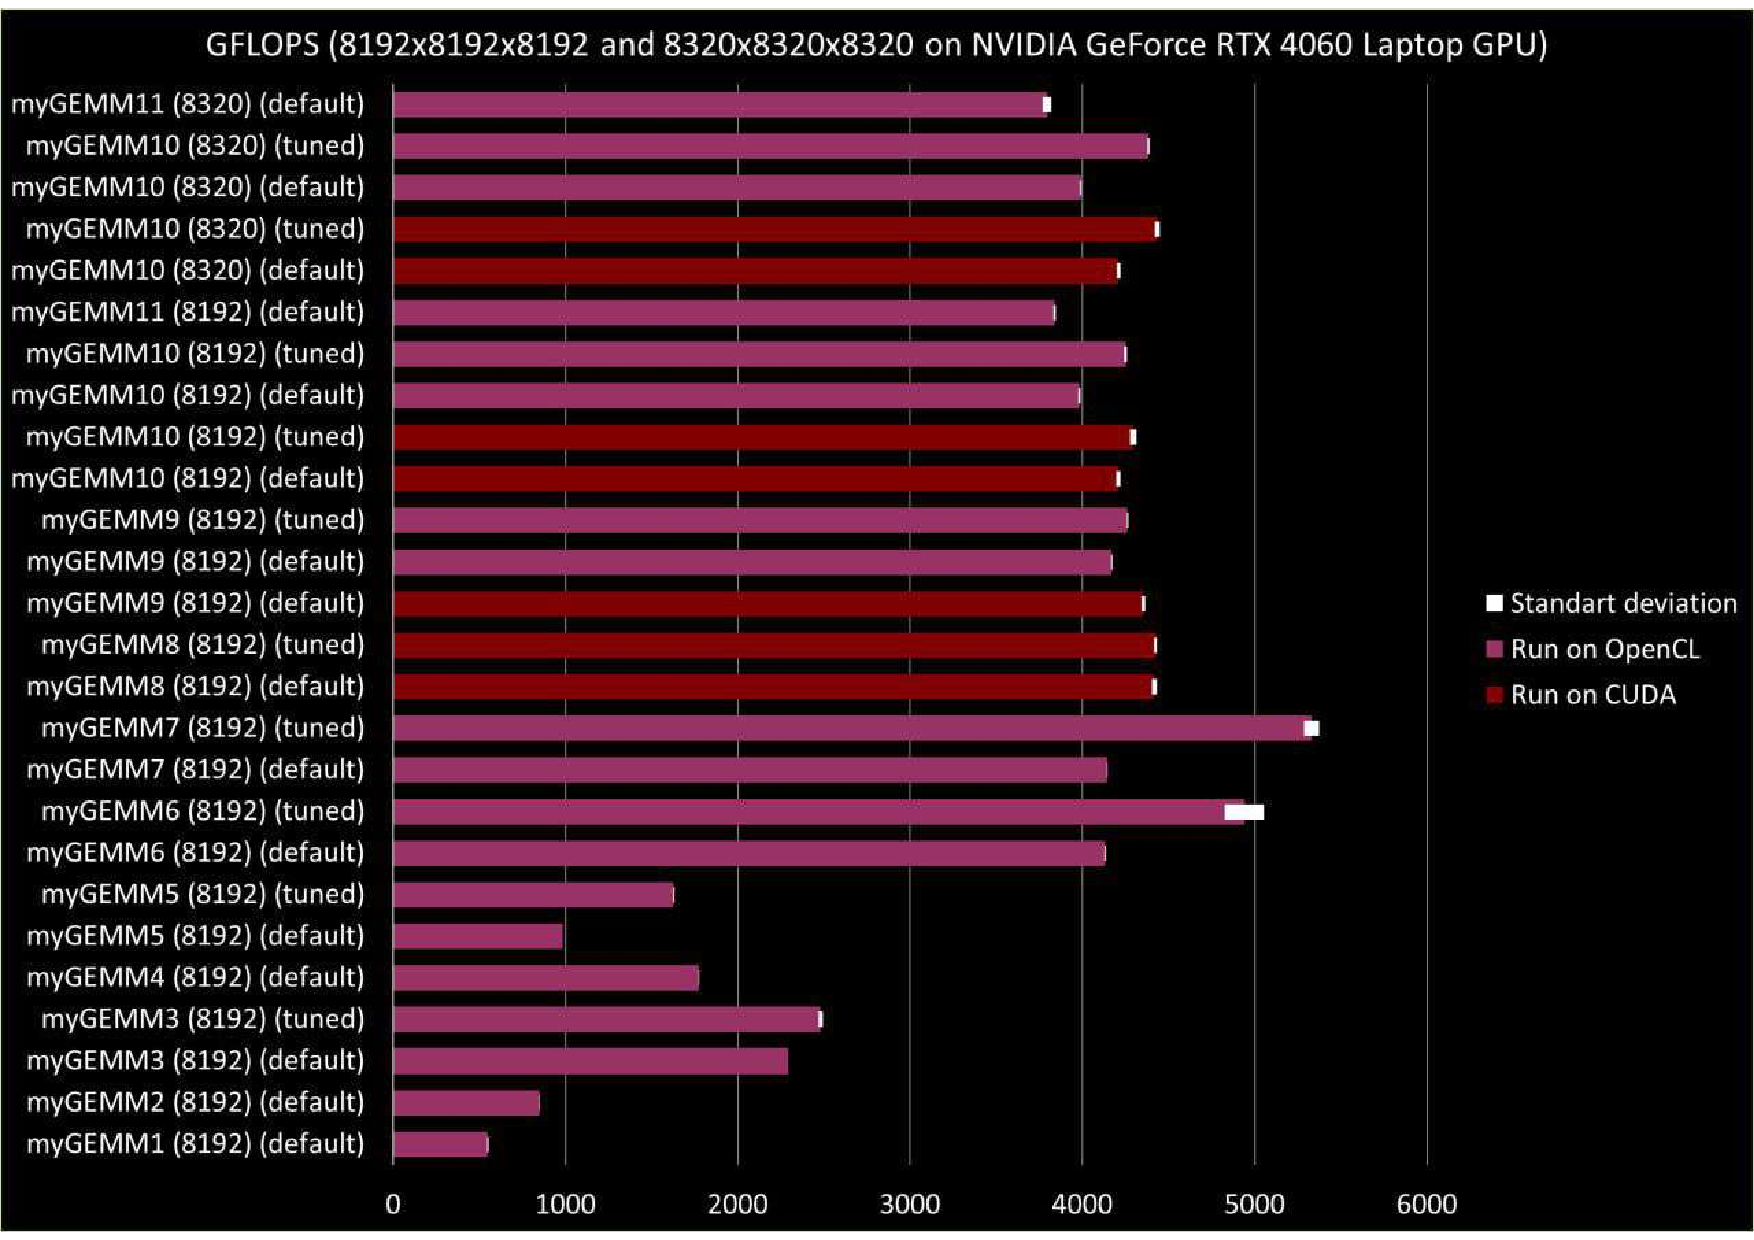
\includegraphics[width=0.57\textwidth]{kernel_comparison.pdf}
    \caption{Производительность вычислительных ядер до и после подбора параметров}
    \label{fig:kernel-comparison}
\end{figure}

В ходе эксперимента были выявлены следующие ядра, показавшие наибольший прирост производительности после оптимизации параметров:

\begin{itemize}
\item ядро 5~--- прирост производительности около 65\% за счет увеличения размера вычислительного блока (TS с 32 до 64) и объема работы на поток (WPT с 8 до 16);
\item ядро 6~--- прирост производительности около 20\% за счет увеличения размера вычислительного блока по измерению K (TSK с 16 до 32);
\item ядро 7~--- прирост произовдительности около 29\% за счет уменьшения ширины вектора (WIDTH с 4 до 2).
\end{itemize}

Остальные ядра (1, 2, 3, 4, 8, 9, 10, 11) не показали заметного изменения производительности, их параметры по умолчанию уже являлись оптимальными или почти оптимальными для используемой видеокарты.

Полученные результаты подтверждают, что учет особенностей конкретного графического процессора при подборе параметров вычислительных ядер позволяет в ряде случаев существенно повысить производительность без изменения алгоритма вычислений.

\section{Заключение}

В ходе выполнения работы получены следующие результаты:

\begin{itemize}
    \item разработаны программы для автоматизированного запуска измерений (\texttt{run\_experiments\_default.py}, \texttt{run\_experiments\_tuned.py}) и статистической обработки результатов (\texttt{calculate\_results\_default.py}, \texttt{calculate\_results\_tuned.py});
    \item написаны модульные тесты для проверки корректности скриптов (\texttt{tests/unit/});
    \item проведены измерения производительности 11 вычислительных ядер в стандартной и оптимизированной конфигурациях на матрицах размером \(8192 \times 8192\) и \(8320 \times 8320\);
    \item выполнен автоматический перебор параметров и определены оптимальные конфигурации для NVIDIA GeForce RTX 4060.
\end{itemize}

Репозиторий: \url{https://github.com/Snaffys/myGEMM}.

Техническая документация, описание методики проведения экспериментов, а также результаты измерений и графики производительности представлены в файле \texttt{README.md} репозитория.

Полученные результаты демонстрируют практическую значимость автоматического подбора параметров вычислительных ядер при разработке высокопроизводительных приложений для графических процессоров. Разработанные средства автоматизации позволяют существенно сократить трудоемкость экспериментальных исследований и могут быть использованы при дальнейшем изучении методов оптимизации вычислений на графических процессорах.
\end{document}
